% ****** Start of file apssamp.tex ******
%
%   This file is part of the APS files in the REVTeX 4.1 distribution.
%   Version 4.1r of REVTeX, August 2010
%
%   Copyright (c) 2009, 2010 The American Physical Society.
%
%   See the REVTeX 4 README file for restrictions and more information.
%
% TeX'ing this file requires that you have AMS-LaTeX 2.0 installed
% as well as the rest of the prerequisites for REVTeX 4.1
%
% See the REVTeX 4 README file
% It also requires running BibTeX. The commands are as follows:
%
%  1)  latex apssamp.tex
%  2)  bibtex apssamp
%  3)  latex apssamp.tex
%  4)  latex apssamp.tex
%
\documentclass[%
 reprint,
%superscriptaddress,
%groupedaddress,
%unsortedaddress,
%runinaddress,
%frontmatterverbose, 
%preprint,
%showpacs,preprintnumbers,
%nofootinbib,
%nobibnotes,
%bibnotes,
 amsmath,amssymb,
 aps,
%pra,
%prb,
%rmp,
%prstab,
%prstper,
%floatfix,
spanish]{revtex4-1}

\usepackage{graphicx}% Include figure files
\usepackage{dcolumn}% Align table columns on decimal point
\usepackage{bm}% bold math
\usepackage{subcaption}
\usepackage[utf8]{inputenc}
\usepackage{tabularx}
%\usepackage{hyperref}% add hypertext capabilities
%\usepackage[mathlines]{lineno}% Enable numbering of text and display math
%\linenumbers\relax % Commence numbering lines

%\usepackage[showframe,%Uncomment any one of the following lines to test 
%%scale=0.7, marginratio={1:1, 2:3}, ignoreall,% default settings
%%text={7in,10in},centering,
%%margin=1.5in,
%%total={6.5in,8.75in}, top=1.2in, left=0.9in, includefoot,
%%height=10in,a5paper,hmargin={3cm,0.8in},
%]{geometry}
\graphicspath{ {imagenes/} }
\begin{document}

\preprint{APS/123-QED}

\title{Percolaci\'on de nodos en redes cuadradas 2d}% Force line breaks with \\
%\thanks{A footnote to the article title}%

\author{A.~Rabinovich}
 %\altaffiliation[Also at ]{}%Lines break automatically or can be forced with \\
\affiliation{%
 Departamento de F\'\i sica, Facultad de Ciencias Exactas y Naturales, Universidad de Buenos Aires,\\
 Pabell\'on I, Ciudad Universitaria, 1428 Buenos Aires, Argentina.
}%

%\collaboration{MUSO Collaboration}%\noaffiliation

\date{\today}% It is always \today, today,
             %  but any date may be explicitly specified

\begin{abstract}
A partir de simulaciones numéricas con redes finitas fue posible reconstruir el comportamiento de las propiedades de una red de nodos bidimensional. Ésta red percola siguiendo una transición de fase de $2^\circ$ orden y sus propiedades son gobernadas por leyes de potencias y exponentes críticos. Se observó un cambio de fase para $p$ cercano al $p_c$ tabulado y fue posible además obtener valores de los exponentes críticos en coincidencia con los teóricos. Finalmente, se estudió el proceso de renormalización basado en la universalidad de las leyes de potencias en redes de tamaño finito en un entorno de la transición.
\end{abstract}


\maketitle

%\tableofcontents

\section{\label{intro}Introducci\'on}
La teoría de percolación es una teoría de transporte y conectividad en sistemas geométricos complejos. Desde hace varios años ésta teoría ha sido utilizada para modelar sistemas desordenados, como propagación de incendios forestales, pozos petrolíferos y difusión en medios desordenados, con resultados que pueden ser obtenidos por medio de relaciones algebráicas simples.\\
Una transición de percolación está caracterizada por un conjunto de exponentes críticos que describen las propiedades de percolación del medio, teniendo en cuenta únicamente el modelo de percolación y la dimensión del espacio, sin que éstas propiedades dependan de detalles microscópicos de las estructuras consideradas. \cite{levinshtein}\cite{stauffer}\cite{havlin}

\section{\label{theory}El modelo}
El modelo teórico de percolación se formula de la siguiente manera. Sea una red periódica infinita, donde cada uno de sus sitios puede estar ocupado con probabilidad $p$ o vacío con probabilidad $1-p$. Dos sitios se consideran conectados si son primeros vecinos. Todos los sitios conectados ya sea directamente o a través de una cadena de sitios conectados, pertenecen al mismo grupo o cluster.\\La teoría de percolación entonces analiza el número y las propiedades de los clusters de una red.\cite{levinshtein}\cite{stauffer}\cite{havlin}

\subsection{\label{transition}Transici\'on de fase}
El problema de percolación requiere encontrar el valor de probabilidad de ocupación crítico $p_c$ para el cual se forma un cluster infinito, o dicho de otra forma, el valor de $p_c$ para el cual el sistema comienza a percolar. Éste es un ejemplo de una transición de fase (o de fenómeno crítico) de segundo orden y mucha de las propiedades del sistema pueden ser descritas de forma sencilla cerca de la transición.

\subsection{\label{critical}Leyes de potencia y exponentes cr\'\i ticos}
Se puede demostrar que para $p=p_c$, se verifica la siguiente relación:
\begin{equation}
\label{ecu:tau}
n_s(p_c)\sim s^{-\tau}
\end{equation}
Con $n_s$ la cantidad por sitio de un cluster de tamaño $s$. El exponente $\tau$ se conoce como exponente de Fisher y es un ejemplo de los llamados exponentes críticos, que controlan las propiedades del sistema cerca de la transición de fase, a través de una ley de potencias.\\
Otras propiedades del sistema que pueden expresarse como leyes de potencias para valores de $p$ cerca de la transición, es decir, tales que $0 < |p-p_c| \ll 1$, son:
\begin{equation}
\label{ecu:beta}
P\sim (p-p_c)^\beta
\end{equation}
Con $P$ la fracción de sitios pertenecientes al cluster percolante. 

\begin{equation}
\label{ecu:gamma}
S(p)\sim (p-p_c)^{-\gamma}
\end{equation}
Con $S$ el tamaño medio de los clusters.\\

\begin{equation}
\label{ecu:nu}
\xi\sim (p-p_c)^{-\nu}
\end{equation}
Con $\xi$ la longitud de correlación y se define como la distancia promedio de dos sitios que pertenecen al mismo cluster. Ésta longitud es entonces el radio de los clusters que contribuyen principalmente a las divergencias de las propiedades del sistema cercano a la transición.\\

Para valores de $p$ cercanos a $p_c$, la ecuación \ref{ecu:tau} puede reescribirse como:

\begin{equation}
\label{ecu:tau2}
n_s(p)=q_0\,s^{-\tau}\,f(z)\ \ \ \ ,\ \ \ \ z=s^\sigma(p-p_c)
\end{equation} 

Donde $\sigma$ es un nuevo exponente crítico que puede relacionarse con los otros mediante:

\begin{equation}
\label{ecu:sigma}
\sigma = \frac{(\tau-2)}{\beta}
\end{equation} 

Estas relaciones que permiten obtener un exponente crítico como función de otros exponentes críticos se conocen como leyes de escala y son fundamentales en la teoría de fenómenos críticos.

La Tabla~\ref{tabla:referencias} resume las principales leyes de potencia obtenidas en la literatura para redes percolantes.\cite{levinshtein}\cite{stauffer}\cite{havlin}\cite{nakanishi}

\begin{table}[h]
\caption{\label{tabla:referencias}%
Valores te\'oricos hallados en la literatura.
}
\begin{ruledtabular}
\begin{tabular}{lll}
%\hline
%\hline
\\[-5pt]
 S\'\i mbolo     & Ley                        & Valor                          \\
\hline
$d$             &   ---                         & $d=2$                        \\
$D$             & $M\sim L^{D}$                 & $D=91/48$                    \\
$\nu$           & $\xi\sim|p-p_c|^{-\nu}$       & $\nu=4/3$                    \\
$\tau$          & $n(p_c)\sim s^{-\tau}$        & $\tau=1+d/D$                 \\
$\sigma$        & $z=s^\sigma(p-p_c)$           & $\sigma=(\nu D)^{-1}$        \\
$\alpha$        & $m_0(p)\sim|p-p_c|^{2-\alpha}$& $\alpha=2-(\tau-1)/\sigma$   \\
$\beta$         & $m_1(p)\sim(p-p_c)^\beta$     & $\beta=\nu(d-D)$             \\
$\gamma$        & $m_2(p)\sim|p-p_c|^{-\gamma}$ & $\gamma=(3-\tau)/\sigma$     \\
%\hline
\end{tabular}
\end{ruledtabular}
\end{table}

\subsection{\label{scaling}Efectos de red finita}
El comportamiento de las redes de tamaño finito (redes cuadradas de lado $L$) se aparta de aquel esperado para sistemas infinitos. Para escalas de longitud mucho menores a $\xi$, es posible ignorar la existencia de $\xi$ finito y el comportamiento del sistema es por lo tanto similar al que se obtendría para $\xi$ infinito. Es decir, en ausencia de una "longitud de referencia", las propiedades relevantes del sistema se comportan como leyes de potencias. \\
Si una cantidad $X$ escaléa cómo $|p-p_c|^{-\chi}$ para $L \gg \xi$, entonces obedece una ley general dada por:
\begin{equation}
\label{ecu:ley_de_escala}
X(L, \xi) \propto \xi^{\frac{\chi}{\nu}} \quad \textrm{si} \quad L \gg \xi
\end{equation} 
\begin{equation}
\label{ecu:ley_de_escala}
X(L, \xi) \propto L^{\frac{\chi}{\nu}} \quad \textrm{si} \quad L \ll \xi
\end{equation} 
Por ejemplo, la masa $M$ del cluster percolante escala como:
\begin{equation}
\label{ecu:masa}
M \propto L^D \quad \textrm{si} \quad L \ll \xi
\end{equation} 
Donde $D$ es una dimensión fractal.

\subsection{\label{renorm}Renormalizaci\'on}
Es posible explotar a\'un m\'as el hecho de que cerca de la transici\'on de fase el sistema se muestra libre de escalas. Todos los clusters o redes cuya longitud lineal sea menor que $\xi$ son similares entre si en promedio. Por lo tanto, cerca de la transición, donde $\xi$ se hace infinito, todas las redes o clusters son similares entre si. Se se toma la mitad de un sistema cerca de la transición, ambos siguen siendo menores que $\xi$ y se parecen en promedio. Si se \emph{re-escala} el sistema, deben seguir siendo v\'alidas las leyes de potencia anteriores.
Entonces, mediante un proceso de \emph{renormalizaci\'on} observaremos que la concentración $p'$ de sitios ocupados en el sistema renormalizado será diferente a la concentración $p$ de la red original. Solo para $p=p_c$ se tiene que $p'=p$. Para una red reescaleada con constante $b$, se obtiene entonces que:
\begin{equation}
\label{ecu:masa}
\xi'=\frac{\xi}{b}
\end{equation} 
y por lo tanto:
\begin{equation}
\label{ecu:masa}
b|p'-p_c|^{-\nu}=|p-p_c|^{-\nu}
\end{equation} 
que es la ecuación básica de renormalización.

\section{\label{simulations}Simulaciones num\'ericas}
Se desarrolló un programa en base al algoritmo de Hoshen-Kopelman para estudiar de forma numérica la teoría de percolación en redes bidimensionales.\cite{Kopelman}
Se estudiaron redes cuadradas bidimensionales de tamaño $L=4, 16, 32, 64, 128, 256$. Los resultados de los distintos exponentes críticos obtenidos y los valores tabulados se observan en la tabla \ref{tabla:resumen}.

\section{\label{results}Resultados}

\subsection{\label{p_c} Determinaci\'on de $p_c$ por diferentes m\'etodos}
Para determinar la probabilidad crítica $P_c$ a partir de la cual el sistema comienza a percolar, se utilizaron diferentes métodos expuestos a continuación:

\subsubsection{Método de bisección}
Comenzando con $p = 0.5$ y una red aleatoria, se verifica si la red percola. En caso de que el sistema percole, se repuebla la red utilizando la misma semilla aleatoria con probabilidad $p = p-\frac{1}{4}$. En caso contrario, se repuebla la red con probabilidad $p = p+\frac{1}{4}$. Ésta operación se repite una cantidad $n$ de veces sumando o restando $\frac{1}{2^k}$ con $k$ el paso actual hasta obtener la precisión deseada.
Para cada $L$ estudiado se generaron $30000$ realizaciones de redes aleatorias y se confeccionó un histograma, figura \ref{fig:histograma1a}, de los valores $P_c$ obtenidos en cada una de ellas.
\begin{figure}[h!]
  \centering
  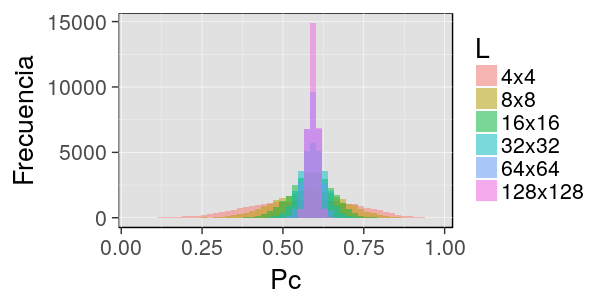
\includegraphics[width=.95\linewidth]{ej1a/histograma}
\caption{Histogramas de probabilidades críticas en función del tamaño de la red cuadrada para 30000 realizaciones de la red.}
\label{fig:histograma1a}
\end{figure}
El valor de $P_c$ se obtuvo entonces como el promedio de los $P_c$ obtenidos en todas las realizaciones, como se observa en la tabla \ref{tabla:tabla1a}.

\begin{table}[h]
\caption{\label{tabla:tabla1a}Valores de $P_c$ promedio para redes de tamaño $L$.}
	\begin{tabular}{c|c}
		\hline
		\hline		
		\\[-5pt]
		$P_c$ & $L$ \\
		\hline
		$0.5\pm0.1$ & $4$ \\
		$0.5\pm0.1$ & $8$ \\
		$0.58\pm0.06$ & $16$ \\
		$0.59\pm0.03$ & $32$ \\
		$0.59\pm0.02$ & $64$ \\
		$0.59\pm0.01$ & $128$ \\															
	\end{tabular}
\end{table}

\subsubsection{Método de la mediana}
Se tomaron $1000$ intervalos de tamaño $\frac{1}{1000}$ para $p$, con $p \in [0, 1]$, y para cada $p$ se calculó la fracción de sistemas que percolaban para $10000$ realizaciones de la red. La figura \ref{fig:probabilidad_acumulada} muestra la fracción de sistemas percolantes en función de $p$ para las distintas redes analizadas. 
\begin{figure}[h!]
  \centering
  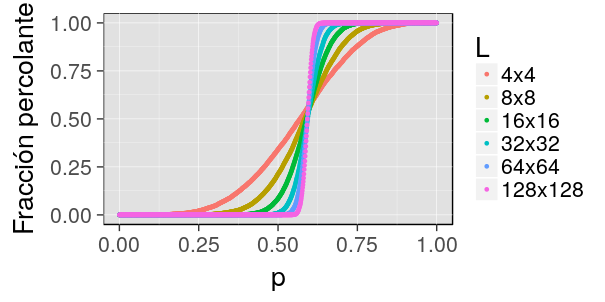
\includegraphics[width=.95\linewidth]{ej1b/probabilidad_acumulada}
\caption{Probabilidad acumulada en función del tamaño de la red cuadrada para 10000 realizaciones de la red para cada p.}
\label{fig:probabilidad_acumulada}
\end{figure}
El $P_c$ se calculó como la probabilidad $p$ tal que al menos la mitad de los clusters percolan. Los resultados se observan en la tabla \ref{tabla:tabla1b}.

\begin{table}[h]
\caption{\label{tabla:tabla1b}Valores de $P_c$ para redes de tamaño $L$.}
	\begin{tabular}{c|c}
		\hline
		\hline		
		\\[-5pt]
		$P_c$ & $L$ \\
		\hline
		$0.569\pm0.005$ & $4$ \\
		$0.584\pm0.004$ & $8$ \\
		$0.590\pm0.004$ & $16$ \\
		$0.593\pm0.004$ & $32$ \\
		$0.592\pm0.004$ & $64$ \\
		$0.593\pm0.004$ & $128$ \\															
	\end{tabular}
\end{table}

En comparación con el método de la bisección, éste método permite obtener mayor precisión en la determinación del $P_c$.

\subsubsection{Determinación de $\nu$}
Para obtener el exponénte crítico $\nu$, partiendo de la ecuación \ref{ecu:nu}, se ajustó en un gráfico log-log de $(<P_c>_l - <P_c>_{\infty})/<P_c>_{\infty}$ en función del lado $L$ de la red, donde $<P_c>_{\infty}$ es el valor tabulado en \cite{stauffer} y $<P_c>_l$ es el $P_c$ obtenido con el método de bisección. La inversa de la pendiente de ésta recta es el exponente $\nu$. La figura \ref{fig:nu} muestra el ajuste realizado para redes de tamaño $L={40, 50, 64, 70, 80, 90, 100, 128, 200}$.
\begin{figure}[h!]
  \centering
  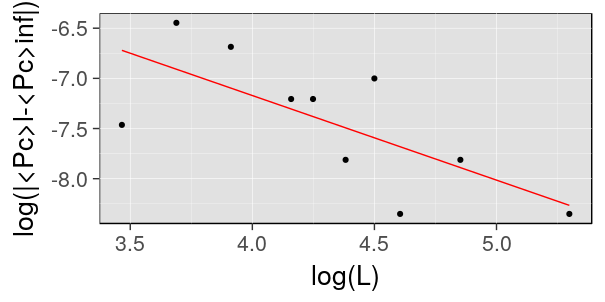
\includegraphics[width=.95\linewidth]{ej1c/nu}
\caption{Gráfico log-log de $(<P_c>_l - <P_c>_{\infty})/<P_c>_{\infty}$ en función del lado $L$ de la red. En rojo el ajuste lineal.}
\label{fig:nu}
\end{figure}
Se encontró mediante éste método $\nu=1.18\pm0.04$ en buena coincidencia con el valor tabulado de $\nu=1.33\pm0.05$.

\subsubsection{\label{1d} Determinación de $P_c$ a partir del ajuste de la distribución de fragmentos}
Para las redes de $L={16, 32, 64, 128}$ se calculó la distribución de fragmentos $n_s$ en función de $s$ para $p\in[0.5, 0.6]$ con intervalos $\Delta p = \frac{1}{4000}$. A partir de la ecuación \ref{ecu:tau}, para cada uno de los $p$ se realizaron $1000$ redes y en un gráfico log-log se ajustó por medio de una función lineal la distribución. Para cada red se obtuvo el $p$ con máximo valor de $R^2$ y se promediaron luego para todas las redes.
La tabla \ref{tabla:tabla1d} muestra los valores obtenidos.

\begin{table}[h]
\caption{\label{tabla:tabla1d}Valores de $P_c$ para redes de tamaño $L$.}
	\begin{tabular}{c|c}
		\hline
		\hline		
		\\[-5pt]
		$P_c$ & $L$ \\
		\hline
		$0.594\pm0.004$ & $16$ \\
		$0.595\pm0.003$ & $32$ \\
		$0.594\pm0.003$ & $64$ \\
		$0.594\pm0.003$ & $128$ \\															
	\end{tabular}
\end{table}

Se observa que coinciden con los valores obtenidos mediante los métodos anteriores dentro del error.

\subsection{\label{2} Intensidad del cluster percolante $P_c$}
Se tomaron $1000$ intervalos de tamaño $\frac{1}{1000}$ para $p$, con $p \in [0, 1]$, y para cada $p$ se calculó la intensidad del cluster percolante $P$ para $1000$ realizaciones de la red. La figura \ref{fig:2} muestra la intensidad $P$ para redes de distinto $L$. A partir de la ecuación \ref{ecu:beta} se ajustó un gráfico log-log $P$ en función de $\epsilon = (p-(p_c)_{\infty})/(p_c)_{\infty}$ por medio de una función lineal para la red $L=128$ y se obtuvo un coeficiente $\beta=0.14\pm0.02$ en concordancia con los valores tabulados.

\begin{figure}[h]
\begin{subfigure}{.25\textwidth}
  \centering
  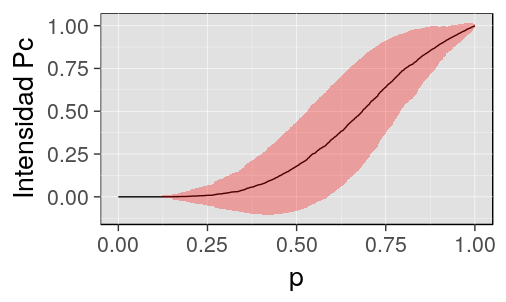
\includegraphics[width=.9\linewidth]{ej2/4x4}
  %\caption{Red cuadrada de 4x4: $\mu=0.569$ $\sigma=0.006$}
  %\caption{Red cuadrada de 4x4: $P_c=0.569\pm0.003$}
  \label{fig:24x4}
\end{subfigure}%
\begin{subfigure}{.25\textwidth}
  \centering
  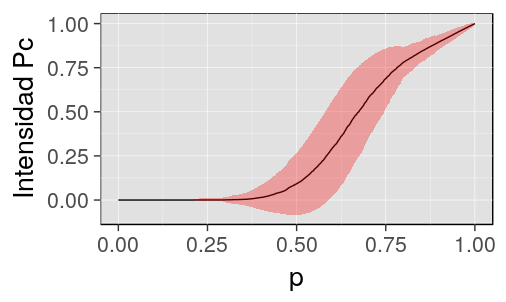
\includegraphics[width=.9\linewidth]{ej2/8x8}
  %\caption{Red cuadrada de 8x8: $\mu=0.584$ $\sigma=0.002$}
  %\caption{Red cuadrada de 8x8: $P_c=0.584\pm0.003$}
  \label{fig:28x8}
\end{subfigure}
\begin{subfigure}{.25\textwidth}
  \centering
  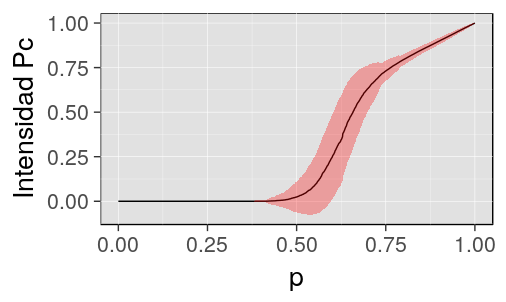
\includegraphics[width=.9\linewidth]{ej2/16x16}
  %\caption{Red cuadrada de 16x16: $\mu=0.589$ $\sigma=0.003$}
  %\caption{Red cuadrada de 16x16: $P_c=0.590\pm0.003$}  
  \label{fig:216x16}
\end{subfigure}%
\begin{subfigure}{.25\textwidth}
  \centering
  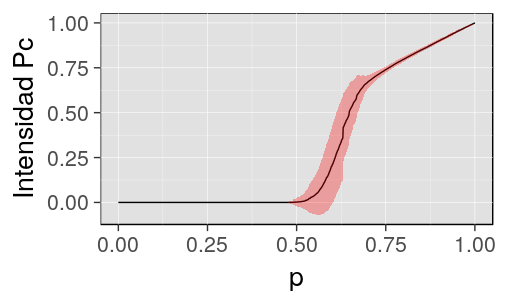
\includegraphics[width=.9\linewidth]{ej2/32x32}
  %\caption{Red cuadrada de 32x32: $\mu=0.593$ $\sigma=0.001$}
  %\caption{Red cuadrada de 32x32: $P_c=0.593\pm0.003$}  
  \label{fig:232x32}
\end{subfigure}
\begin{subfigure}{.25\textwidth}
  \centering
  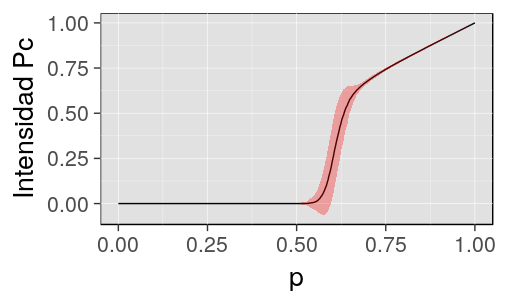
\includegraphics[width=.9\linewidth]{ej2/64x64}
  %\caption{Red cuadrada de 64x64: $\mu=0.5927$ $\sigma=0.0006$}
  %\caption{Red cuadrada de 64x64: $P_c=0.592\pm0.003$}  
  \label{fig:264x64}
\end{subfigure}%
\begin{subfigure}{.25\textwidth}
  \centering
  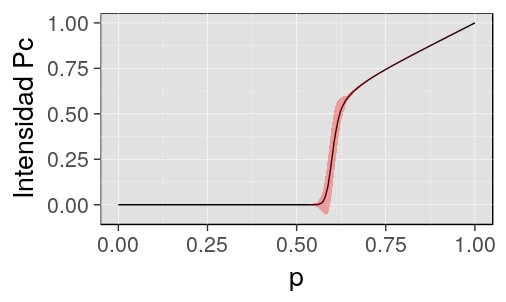
\includegraphics[width=.9\linewidth]{ej2/128x128}
  %\caption{Red cuadrada de 128x128: $\mu=0.5931$ $\sigma=0.0005$}
  %\caption{Red cuadrada de 128x128: $P_c=0.593\pm0.003$}  
  \label{fig:2128x128}
\end{subfigure}
\caption{Intensidad del cluster percolante en función de p y del tamaño de la red cuadrada para 1000 realizaciones de la red.}
\label{fig:2}
\end{figure}


\subsection{\label{3} Determinaci\'on de la dimensi\'on fractal $D$ }
Para determinar la dimensión fractal se tomó $p=(p_c)_{\infty}$ y se midió la masa $M$ del cluster percolante en función de $L={4,...,128}$. La figura \ref{fig:3} muestra en escala logarítmica la masa del cluster percolante como función de $L$. La recta de ajuste permitió obtener un valor de $D=1.840\pm0.001$ con un valor de $R^2=0.9999$, similar al valor tabulado de $D=1.89$.
\begin{figure}[h]
  \centering
  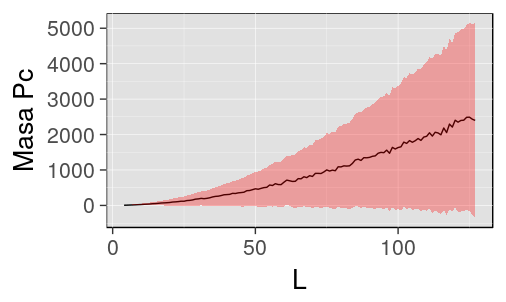
\includegraphics[width=.9\linewidth]{ej3/masa}
  \label{fig:2masa}
\caption{Masa del cluster percolante $P_c$ en función del tamaño de la red cuadrada en escala logarítmica para 10000 realizaciones de la red y recta de ajuste.}
\label{fig:3}
\end{figure}

\subsection{\label{4} Hipótesis de scaling }
Para encontrar la forma cualitativa de la función de scaling $f(z)$, se obtuvo $n_s$ en función de $p \in [0, 1]$ para una red de $L=64$.
Utilizando $\tau=1.74$ y $q_0=exp(-4)$ encontrados en la sección \ref{1d}, se obtuvo $(n_s)_c$. Para el cálculo de $z=s^\sigma\epsilon$, se utilizó $\sigma_{\infty}=36/91$. A partir de la ecuación \ref{ecu:tau2}, se graficó entonces $\frac{n_s}{(n_s)_c}$ en función de $z$ para aquellos fragmentos que cumplieran que $0.01 < \frac{s}{s_0} < 0.12$ con $s_0$ el tamaño del cluster percolante.
\begin{figure}[h]
  \centering
  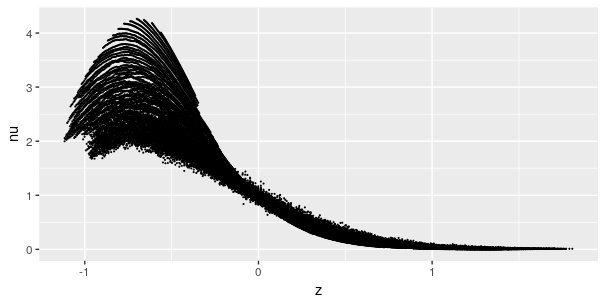
\includegraphics[width=.9\linewidth]{ej4/scaling}
\caption{Función de scaling $f(z)$}
\label{fig:4}
\end{figure}
La figura \ref{fig:4} muestra la forma cualitativa de la función de scaling.

\subsection{\label{5} Exponente $\sigma$}
Para cada valor de $s$ tal que $1 < s < 16$, graficamos $n_s$ en función de $\epsilon=\frac{(p-p_c)}{p_c}$, figura \ref{fig:5ns_vs_e}, obteniendo la $p_{max}(s)$ que maximiza la producción de fragmentos de tamaño $s$. Ajustando luego el gráfico log-log de $p_{max}-p_c$ en función de $s$ por una recta, como se observa en la figura \ref{fig:5sigma}, se obtuvo un valor de $\sigma=0.386\pm0.005$, cercano al valor tabulado de $\sigma=0.395$.

\begin{figure}[h]
  \centering
  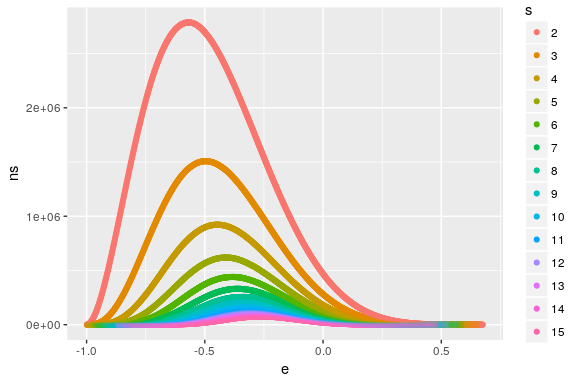
\includegraphics[width=.9\linewidth]{ej5/ns_vs_e}
\caption{$n_s$ en función de $\epsilon=(p-p_c)/p_c$}
\label{fig:5ns_vs_e}
\end{figure}

\begin{figure}[h]
  \centering
  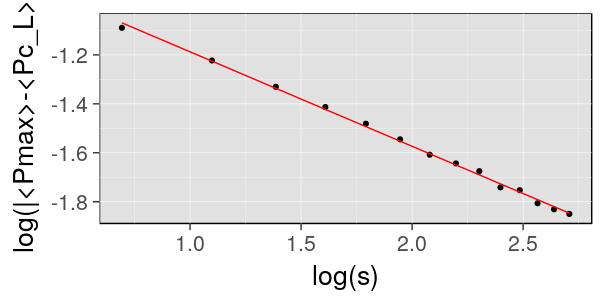
\includegraphics[width=.9\linewidth]{ej5/sigma}
\caption{$p_{max}-p_c$ en función de $s$ en escala logarítmica y ajuste lineal}
\label{fig:5sigma}
\end{figure}


\subsection{\label{6} $\gamma$-matching}
Para una red de $L=256$ y valores de $p\in[0.4, 0.7]$ se obtuvo el segundo momento de la distribución $M2$ en función de $\epsilon$, cómo se observa en la figura \ref{fig:6m2}. Luego se encontró el máximo y a partir de ese punto se realizó un ajuste lineal hacia la derecha y hacia la izquierda de la curva, tomando distinta cantidad de puntos, en escala log-log. La pendiente de cada curva es un posible exponente $\gamma$, y aquel donde se intersecan los exponentes de los $\epsilon$ positivos y negativos puede ser considerado como $\gamma$. La figura \ref{fig:6gamma} muestra los distintos valores de $\gamma$ para los distintos $\epsilon$, siendo $\gamma=1.85$ donde se cruzan. Éste valor obtenido está lejos del tabulado, $\gamma_t=2.38$. Se observó además que dependiendo del máximo que se utilice, se pueden obtener distintos valores de $\gamma$, por lo que éste método no serviría para calcular $\gamma$. Es posible que esto se deba a efectos de red finita, ya que el $\epsilon$ del máximo que se encuentra no es necesariamente el valor para el cual $M2$ diverge.

\begin{figure}[h]
  \centering
  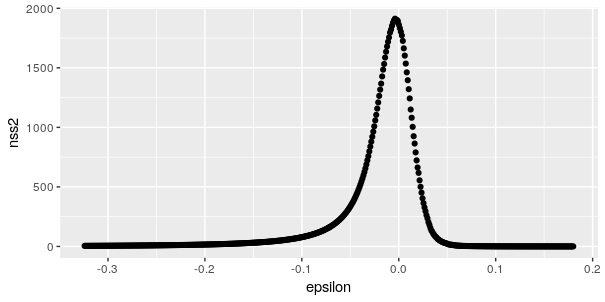
\includegraphics[width=.9\linewidth]{ej6/m2}
\caption{$n_s$ en función de $\epsilon=(p-p_c)/p_c$}
\label{fig:6m2}
\end{figure}

\begin{figure}[h]
  \centering
  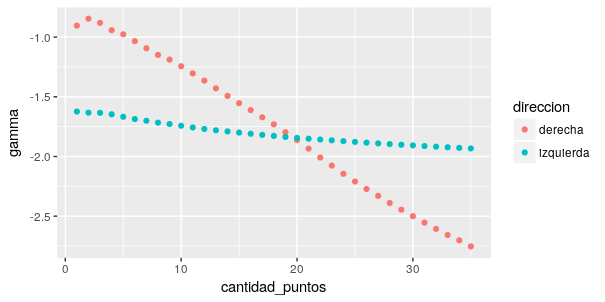
\includegraphics[width=.9\linewidth]{ej6/gamma}
\caption{$p_{max}-p_c$ en función de $s$ en escala logarítmica y ajuste lineal}
\label{fig:6gamma}
\end{figure}

\section{\label{R} Verificaci\'on de resultados por renormalizaci\'on}

Podemos verificar, al menos de manera aproximada, los resulados del las secciones realizando un proceso de renormalzaci\'on de \emph{celda peque\~na}. Consideramos un porci\'on de red de lado $b=2$ y la llamamos un \emph{super-nodo}. Luego, se debe elegir una regla para renormalizar. Por ejemplo, utilizando mayoría simple. Si tres o cuatro de los cuatro nodos del super nodo está ocupado, diremos que el super nodo está ocupado. Si por el contrario, menos de tres nodos del super nodo están vacantes, diremos que el super nodo está vacante. Entonces, la probabilidad de ocupación $p'$ del super nodo será:
\begin{equation}
\label{ecu:renormalizacion_mayoria}
4p^3(1-p) + p^4 = p'
\end{equation} 
porque la probabilidad de encontrar tres nodos ocupados y uno vacío es $p^3(1-p)$ y hay cuatro configuraciones posibles de trens nodos ocupados, mientras que la probabilidad de encontrar todos ocupados es $p^4$.\\
Para $p=p_c$, vale que $p'=p$ y es por lo tanto un punto fijo (su valor no cambia frente a la renormalización). Las soluciones del polinomio son $p_1=1$ y $p_2=0.76$, ambas lejos del valor de $p_c=0.5927$ tabulado. Sin embargo, un valor de $p>p_c$ era esperable, ya que los nuevos clusters serán más gruesos que los anteriores.\\
De ésta forma, a partir de reglas de renormalización y puntos fijos, es posible construirse nuevas redes cuyos exponentes críticos, en principio, serían similares a los originales.

\section{\label{conclusions}Conclusiones}
La Tabla \ref{tabla:resumen} resume los resultados obtenidos para redes cuadradas de distinto tamaño y los compara con los valores tabulados hallados en la bibliografía. Se observa que en la mayor parte de los casos los resultados obtenidos se encuentran en concordancia con los tabulados, con excepción del valor de $\gamma$.

\begin{table}[h]
\caption{\label{tabla:resumen}%
Valores obtenidos mediante simulación y los correspondientes te\'oricos hallados en la literatura.
}
\begin{ruledtabular}
\begin{tabular}{llll}
%\hline
%\hline
\\[-5pt]
 S\'\i mbolo     & Ley                        & Valor Tabulado  & Valor obtenido \\
\hline
$d$             &   ---                         & $d=2$                       & $d=2$ \\
$D$             & $M\sim L^{D}$                 & $D=1.89$                    & $D=1.840\pm0.001$\\
$\nu$           & $\xi\sim|p-p_c|^{-\nu}$       & $\nu=1.33$                  & $\nu=1.18\pm0.04$\\
$\tau$          & $n(p_c)\sim s^{-\tau}$        & $\tau=2.05$                 & $\tau=2.08\pm0.0005$\\
$\sigma$        & $z=s^\sigma(p-p_c)$           & $\sigma=0.395$              & $\sigma=0.386\pm0.005$\\
$\beta$         & $m_1(p)\sim(p-p_c)^\beta$     & $\beta=0.14$                & $\beta=0.14\pm0.02$\\
$\gamma$        & $m_2(p)\sim|p-p_c|^{-\gamma}$ & $\gamma=2.38$               & $\gamma=1.85$\\
%\hline
\end{tabular}
\end{ruledtabular}
\end{table}

A partir de simulaciones numéricas con redes finitas fue posible reconstruir el comportamiento de las propiedades del sistema percolante gobernadas por leyes de potencias y exponentes críticos. Se observó un cambio de fase para $p$ cercano al $p_c$ tabulado y fue posible además obtener valores de los exponentes críticos en coincidencia con los teóricos. Finalmente, se estudió el proceso de renormalización basado en la universalidad de las leyes de potencias en redes de tamaño finito en un entorno de la transición.

\begin{acknowledgments}
A. Rabinovich es becario doctoral del CONICET.\\
Los códigos fuentes en lenguaje C y el análisis de resultados en lenguaje R pueden encontrarse para su descarga en https://github.com/andresrabinovich/fisica\_computacional
\end{acknowledgments}

\appendix
%\bibliography{apssamp}% Produces the bibliography via BibTeX.
\bibliography{informe}% Produces the bibliography via BibTeX.

\end{document}
%
% ****** End of file apssamp.tex ******
